\documentclass[twocolumn]{article}
\usepackage{amsmath}
\usepackage{graphicx}
\usepackage{hyperref}
\title{Factoring with $n+2$ clean qubits and $n-1$ dirty qubits}
\author{Craig Gidney}

\begin{document}
\maketitle

\begin{abstract}
\em
We present asymptotically size-efficient reversible classical circuits for performing various arithmetic operations aided by ancilla in an unknown state.
We improve the number of qubits needed to factor an $n$-bit number with Shor's algorithm \cite{Shor1999} from $2n+2$ clean qubits \cite{takahashi2006, haner2016} to $2n+1$ qubits, $n-1$ of which can be an unknown state, without increasing the asymptotic size or depth of the circuit.
\end{abstract}

\section{Introduction}

When constructing quantum circuits, or classical reversible circuits, an important resource is the number of available ancilla.
An ancilla is an extra bit or qubit available for use by a circuit as temporary workspace.
Ancilla may be initialized to a known state (``clean bit"), or be given to the circuit in an unknown state (``dirty bit") that must be restored before the circuit finishes.
Clean bits are more valuable, allowing for simpler and more compact circuit constructions, but dirty bits are more plentiful, since any temporarily unused bit is a borrowable dirty bit.

Because one part of a circuit can borrow dirty bits from another part of the same circuit, circuit constructions that require only dirty bits are easier to apply under tight space constraints, or on circuit topologies where other ancilla are too far away to be acquired quickly.
When attempting to reduce the number of bits or qubits required by a circuit, converting clean ancilla to dirty ancilla makes a useful intermediate goal.
In this paper, at great cost to the constant factors in the gate count and depth, we reduce the number of qubits required to perform period finding from $2n+2$ clean qubits \cite{takahashi2006, haner2016} to $n+2$ clean qubits and $n-1$ dirty qubits without increasing the asymptotic costs.

Our paper is structured as follows.
The introduction describes the various sections and also itself for no discernible reason.
In section \ref{sec:construct} we iteratively reduce period finding into simpler and simpler arithmetic operations, until we reach constant-sized gates, while tracking the number of required dirty ancilla.
Then, in section \ref{sec:costs}, we discuss the novelty and comparative costs of the presented arithmetic circuit constructions.
Finally, section \ref{sec:conclusion} concludes and summarizes.

All constructions assume a 2s-complement representation of integers.
Multi-qubit arithmetic operations always have the least significant bit towards the top.
For clarity, circuit diagrams will divide operations into separate input and output parts, with inputs shaded gray, when applicable.
For completeness, even when the period finding reduction doesn't produce a controlled version of an operation, we provide controllable constructions of that operation that scale well with the number of controls.


\section{Period Finding into Toffolis} \label{sec:construct}

\subsection{Period Finding}

A high-level circuit for period finding, the core quantum subroutine of Shor's quantum factoring algorithm \cite{Shor1999}, is shown in figure \ref{fig:period-finding}.

Because period-finding measures all qubits immediately after performing a quantum Fourier transform, most of the transformed qubits can be measured earlier than shown.
In fact, each qubit can be measured so early that the next does not even need to be initialized yet!
Only one of the qubits in the phase-estimation register needs to be present at a time, and so the phase register can be reduced to a single repeatedly-used qubit \cite{beauregard2003}.
Figure \ref{fig:period-finding-solo-phase-qubit} shows a period-finding circuit with this property.

The period-finding circuit in figure \ref{fig:period-finding-solo-phase-qubit} is our high-level starting point.
It uses (a) controlled modular multiplication, (b) measurement, (c) X-axis rotations parametrized by previous measurements, and (d) qubit resets.
The only non-trivial operation is (a), the controlled modular multiplication of an $n$-qubit register (requiring $n-1$ dirty ancilla and 1 clean ancilla using our constructions).

We perform modular multiplication with multiply-accumulates and a second clean register as in \cite{beauregard2003}.
However, to allow the second register to be dirty, it is convenient to pair each modular multiplication with an inverse and negated multiplication on another register.
We will refer to this combined operation as a ``bimultiply".

Note that we must preserve the state of the second register, but bimultiplication trashes that state with many multiplications by unknown constants.
However, because the first register is initialized to store 1 and gets multiplied by constants inverse to the ones trashing the second register, we can fix the second register by measuring the first register and using its value to perform a clean-up bimultiplication after the usual end of the circuit.
Figure \ref{fig:period-finding-solo-phase-qubit-explicit-dirty-register} shows this construction.

If the second register contained a value larger than $R$, it would end up trashed despite the final clean-up operation.
Our modular circuit constructions do not guarantee that out-of-range values (i.e. values not below the modulus $R$) are well behaved.
To avoid this problem, we require that the registers have minimal size $n = \lceil \lg_2(R-1) \rceil$ and that the second register's most-significant-bit (MSB) be a clean qubit initialized to zero.

\begin{figure}
  \centering
  \makebox[\linewidth]{
    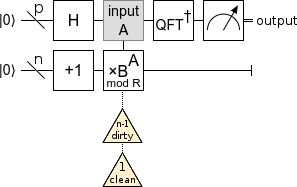
\includegraphics[width=\linewidth]{assets/shor-period-finding.png}
  }
  \caption{\em
	High-level period finding circuit \cite{Shor1999}.
	$R$ is the modulus being queried, $B$ is a randomly chosen base, $n$ is the number of bits needed to store $R$, and $p \in \Theta(n)$ controls the precision of the phase estimation step.
    The triangles indicate how many ancilla are needed ``behind the scenes", by our constructions, to perform an operation.
	Recovering the period requires classically processing the sampled output with a continued fractions algorithm.
  }
  \label{fig:period-finding}
\end{figure}

\begin{figure*}
  \centering
  \makebox[\linewidth]{
    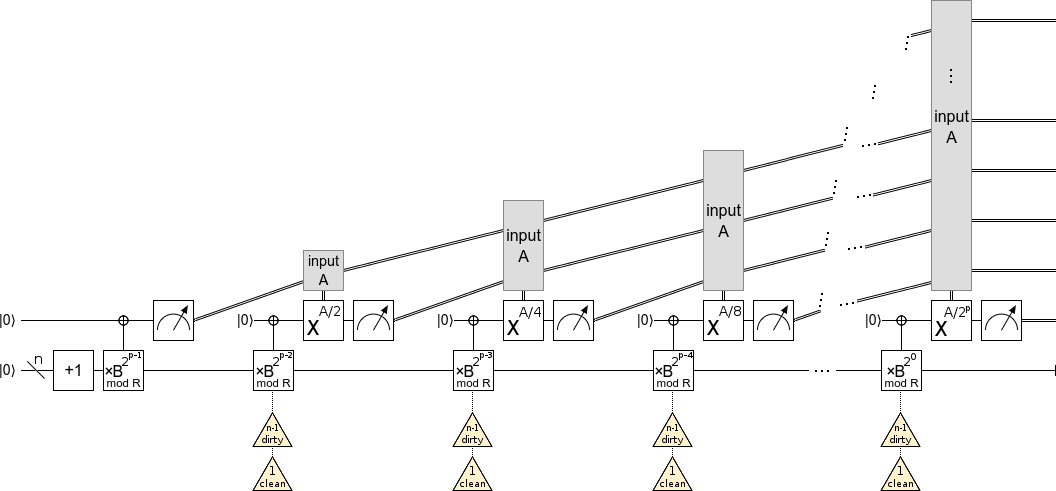
\includegraphics[width=\linewidth]{assets/shor-period-finding-solo-phase-qubit.png}
  }
  \caption{\em
	Period finding with a single phase-estimation qubit \cite{beauregard2003}.
	The small oplus' ({\tiny $\oplus$}) are ``X-axis controls".
	An X-axis control is equivalent to a normal control, but with a Hadamard gate applied before and after.
	It conditions on the state $\frac{1}{\sqrt 2}|0\rangle - \frac{1}{\sqrt 2}|1\rangle$ instead of on the state $|1\rangle$.
  }
  \label{fig:period-finding-solo-phase-qubit}
\end{figure*}

\begin{figure*}
  \centering
  \makebox[\linewidth]{
    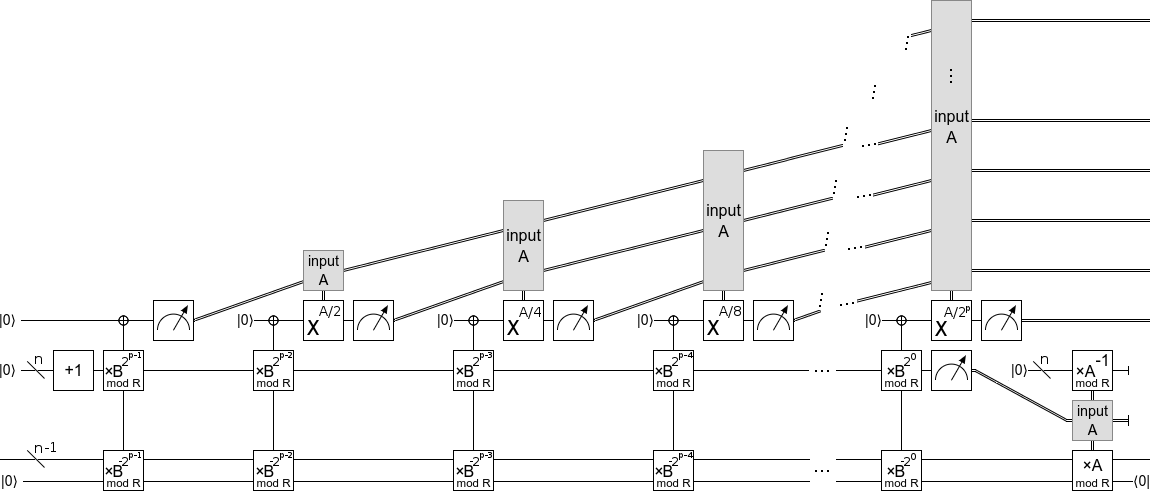
\includegraphics[width=\linewidth]{assets/shor-period-finding-solo-phase-qubit-double-register.png}
  }
  \caption{\em
	Period finding with a single phase-estimation qubit and paired inverse multiplications.
	The terminating bra $\langle 0 |$ indicates that the bottom wire will always end up in the state $|0\rangle$, without post-selection.
  }
  \label{fig:period-finding-solo-phase-qubit-explicit-dirty-register}
\end{figure*}


\subsection{Modular Bimultiplication}

As in \cite{beauregard2003}, we perform controlled modular multiplication with a second register and modular scaled-multiply-accumulates operations.
However, because the second register is dirty, we need three scaled-multiply-accumulates instead of the usual two.

As with all other modular arithmetic circuits in this paper, we make no guarantees about the circuit's behavior when either of the input registers is out of range (i.e. have values not below $R$).

Suppose that the two registers start in the state $(a, b)$, working modulo $R$.
By multiply-adding the first register times $K$ into the second register, the system advances to $(a, b+aK)$.
Then a multiply-subtract times $K^{-1}$ out of the first register puts the system into the state $(a-bK^{-1}-aKK^{-1}, b+aK)$, which is just $(-bK^{-1}, b+aK)$.
Next, we cancel the $b$ term in the second register by multiply-adding the first register times $K$ into it again, leaving $(-bK^{-1}, b+aK-bK^{-1} \cdot K)$ which is simply $(-bK^{-1}, aK)$.
Finally, we swap to $(aK, bK^{-1})$.
The overall effect is to multiply the first register by $K$ and the second register by $-K^{-1}$, as desired.
See figure \ref{fig:controlled-modular-multiply} for the circuit diagram.

In the case where $K$ has no multiplicative inverse modulo $R$, this construction will not work (it would define an invalid irreversible operation).
However, that would mean $K$ is a factor of $R$, a case which the very lucky user can check and handle classically before invoking a quantum period finding circuit.

\begin{figure}
  \centering
  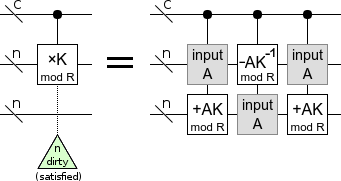
\includegraphics[width=\linewidth]{assets/controlled-modular-multiply.png}
  \caption{\em
    Performing a modular bimultiplication with three scaled-multiply-accumulates and a swap.
    $K$ must have a multiplicative inverse modulo $R$.
  }
  \label{fig:controlled-modular-multiply}
\end{figure}


\subsection{Modular Scaled-Multiply-Accumulation}

To perform scaled-multiply-accumulation, we use a shift-and-add approach similar to \cite{beauregard2003}.
We right-shift (i.e. divide by $2 {\pmod R}$) the target register $n-1$ times, then begin iteratively left-shifting (i.e. multiplying it by 2) and adding $K$ into the target conditioned on the most significant bit of the input, then the next most significant bit, and so forth.
(The more significant bits go first because their effects must be hit by more left-shifts.)
See figure \ref{fig:controlled-modular-multiply-accumulate}.

The conditional offset operations need one dirty bit, and the modular doubling need two, but there are more than enough unused bits available to borrow, so the circuit as a whole doesn't require any dirty bits.

Note that the modular doublings require $R$ to be odd, since otherwise the operation would be irreversible and non-unitary.
However, given that in the intended use case $R$ is a number to be factored, it is reasonable to require callers to have factored out multiples of two beforehand.

\begin{figure}
  \centering
  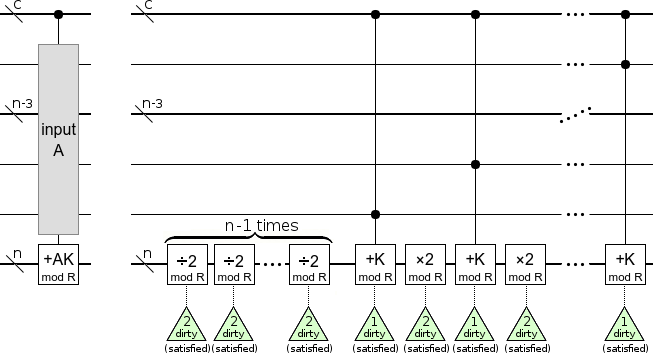
\includegraphics[width=\linewidth]{assets/controlled-modular-multiply-accumulate.png}
  \caption{\em
    Reducing a modular multiply-accumulate into the modular equivalent of shift-and-add.
    Assumes $R$ is odd.
  }
  \label{fig:controlled-modular-multiply-accumulate}
\end{figure}


\subsection{Modular Doubling}

To multiply a register by 2 modulo an odd $R$, we use pivot-flips (see section \ref{sec:pivot-flips}) and subtraction to align the two halves of the input space on the MSB boundaries.
Then we finish the job with a left-rotate.
See figure \ref{fig:modular-double}.

To invert the doubling, i.e. to divide by 2 instead of multiplying by 2, recurse and reverse: invert each operation in the construction, then apply the operations in reverse order. 
Except for period finding, all circuits presented in this paper can be inverted (e.g. from addition to subtraction) with recurse-and-reverse.

\begin{figure}
  \centering
  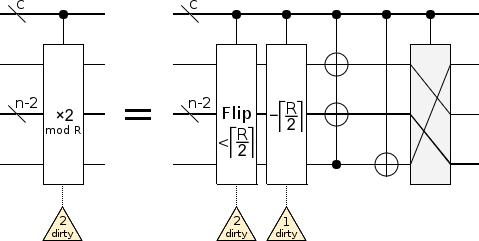
\includegraphics[width=\linewidth]{assets/controlled-modular-double.png}
  \caption{\em
    Controlled modular doubling in $O(c + n \lg n)$ gates, $O(c + n)$ depth, with 2 dirty ancilla.
    $R$ must be odd.
  }
  \label{fig:modular-double}
\end{figure}


\subsection{Modular Addition / Offset}

As shown in figure \ref{fig:mod-add-from-pivot-flip-bars}, a modular addition is three pivot-flips (see section \ref{sec:pivot-flips}).
To add $A$ into a register modulo $R$, perform pivot-flips with the pivot at $R-A$, then $R$, then $A$.
See figure \ref{fig:controlled-modular-add} for the circuit.

Interestingly, modular addition only requires a dirty bit if it's {\em not} controlled.
And when performing modular offset (i.e. adding a compile-time constant to a register), {\em two} dirty bits are required whether or not the operation is controlled.
See figure \ref{fig:controlled-modular-offset}.

\begin{figure}
  \centering
  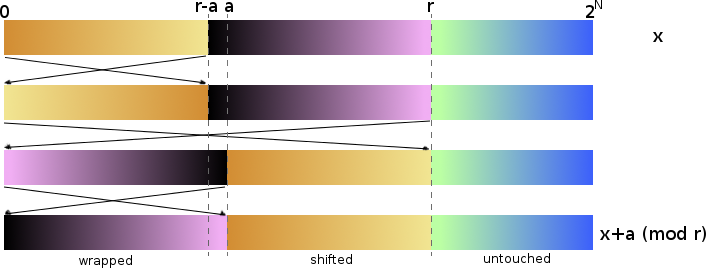
\includegraphics[width=\linewidth]{assets/mod-add-from-pivot-flip-bars.png}
  \caption{\em
     Modular addition of $A \pmod{R}$ can be done with three pivot flips.
     One at $R-A$, then one at $R$, then one at $A$.
     Requires $A \leq R$ (or else the operation will trash the target).
   }
  \label{fig:mod-add-from-pivot-flip-bars}
\end{figure}

\begin{figure}
  \centering
  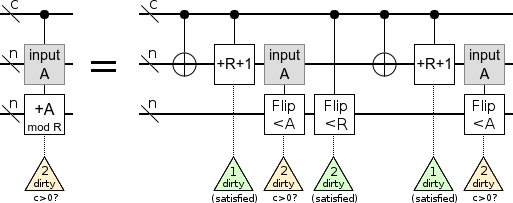
\includegraphics[width=\linewidth]{assets/controlled-modular-addition.png}
  \caption{\em
    Controlled modular addition.
    The circuit as a whole only needs a dirty bit if no control qubits are available to be borrowed by the uncontrolled pivot-flip operations.
  }
  \label{fig:controlled-modular-add}
\end{figure}

\begin{figure}
  \centering
  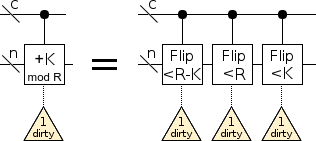
\includegraphics[width=\linewidth]{assets/controlled-modular-offset.png}
  \caption{\em
    Controlled modular offset.
  }
  \label{fig:controlled-modular-offset}
\end{figure}


\subsection{Pivot-Flips} \label{sec:pivot-flips}

We implemented both modular doubling and modular offset/addition in terms of a non-standard operation we call ``pivot-flips".
A pivot-flip is an operation that reverses the order of states less than a given pivot value, without affecting other states.
For example, a pivot-flip with the pivot equal to 4 would swap $|0\rangle$ and $|3\rangle$, swap $|1\rangle$ and $|2\rangle$, and leave all other states untouched.

The exact permutation performed by a pivot-flip with pivot equal to $A$ is:

$$\text{PivotFlip}_A = \sum_{i=0}^{A-1} |A-i-1\rangle \langle i| + \sum_{i=A}^{N-1} |i\rangle \langle i|$$

To perform a pivot-flip efficiently, we use the fact that $x \rightarrow \lnot(x - A)$ nearly does what is required: it flips the range below $A$ but unfortunately also flips the range above-and-including $A$.
However, because $x \rightarrow \lnot(x - A)$ is its own inverse, the operation can be ``toggle-controlled'': unless a controlling qubit is toggled between two applications of the operation, it will have no effect or undo itself.
Also, because the operation doesn't change whether a given value is below the pivot, the controlling qubit can be toggled by a comparison of the {\em target} against the pivot $A$.
See figure \ref{fig:controlled-pivot-flip} for the construction.
For states that are less than the pivot $A$, the comparison is true, the ancilla is toggled both times, and exactly one of the controlled subtract-and-inverts will fire.
For other states, the ancilla does not change and so the subtract-and-inverse happens either no times or two times (undoing itself) for a net effect of no effect.

Note that, depending on whether or not the pivot is a compile-time constant or another qubit register, different subtraction constructions are used when reducing further.
This distinction matters because the constant-offset case uses $O(n \lg n)$ gates \cite{haner2016} instead of the $\Theta(n)$ gates used by enregistered addition \cite{takahashi2005}.
Also, the constant-offset case requires an extra dirty bit (unless quantum operations are used, e.g. see figure \ref{fig:bootstrap-ancilla}).

\begin{figure}
  \centering
  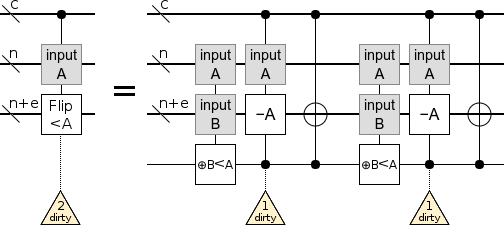
\includegraphics[width=\linewidth]{assets/controlled-pivot-flip.png}
  \caption{\em
    Controlled pivot-flip circuit with an enregistered pivot.
  }
  \label{fig:controlled-pivot-flip}
\end{figure}

\begin{figure}
  \centering
  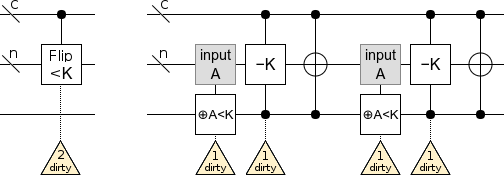
\includegraphics[width=\linewidth]{assets/controlled-const-pivot-flip.png}
  \caption{\em
    Controlled pivot-flip circuit with a constant pivot.
    The extra dirty ancilla, compared to the enregistered case, comes from the controlled-offset construction.
  }
  \label{fig:controlled-pivot-flip}
\end{figure}

\begin{figure}
  \centering
  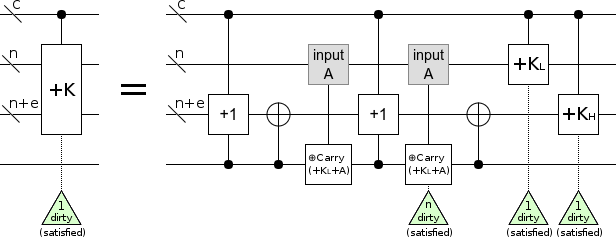
\includegraphics[width=\linewidth]{assets/controlled-offset.png}
  \caption{\em
      Offset circuit from \cite{haner2016}, but modified to include controls.
      Uses $O(n \lg n)$ gates and $O(n)$ depth (by overlapping the recursive cases).
      Note that, if $c$ is not $O(1)$, the recursion introduces additional non-linear costs.
  }
  \label{fig:controlled-offset}
\end{figure}


\subsection{Comparison}

Comparison operations toggle a target bit based on the relationship between two input registers.
We implement comparisons as in \cite{takahashi2005}, using an addition followed by a subtraction that is slightly smaller to clear all changes except an overflow signal into the target.
See figures \ref{fig:comparison-less} and \ref{fig:comparison-less-const}.

To perform a $\leq$ instead of a $<$, simply add/subtract $A+1$ instead of $A$.
(Apply the extra increment/decrement to the target register, not the input register, since incrementing the input register may wrap it to zero.)

Beware that, in these constructions, if the $B$ register is smaller than the $A$ register, the high bits of $A$ are lost and the construction breaks.
To fix the problem, swap the roles of A and B (i.e. subtract out of A instead) and use the opposite comparison.
Alternatively, any operations generated by the subtraction or decrement gates that toggle the target bit can be controlled by the high bits of $A$ all being off and otherwise (if any of the high bits are on) concluding $A>B$ and toggling the result bit as appropriate for the comparison being implemented.

\begin{figure}
  \centering
  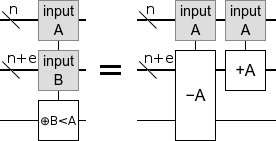
\includegraphics[width=\linewidth]{assets/comparison-less.png}
  \caption{\em Toggling a target bit if one register is less than another, without using ancilla.}
  \label{fig:comparison-less}
\end{figure}

\begin{figure}
  \centering
  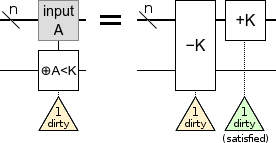
\includegraphics[width=\linewidth]{assets/comparison-less-const.png}
  \caption{\em Toggling a target bit if a register is less then a constant, using a dirty ancilla and $O(n \lg n)$ gates.}
  \label{fig:comparison-less-const}
\end{figure}


\subsection{Addition / Offset}

In \cite{van2004}, a reversible adder with $O(N)$ depth and $O(N)$ size, requiring a single clean ancilla, is described.
If the ancilla is not initialized in the off state, the target register ends up storing $a+b+1$ instead of $a+b$.
For clarity, we review how to elide the ancilla.

The need for the ancilla to be clean can be fixed by inverting (bitwise-NOT-ing) the input and target registers before and after the addition when the ancilla is on.
Because $\lnot x = -x-1$, and the registers are the same size, temporarily inverting the target effectively turns the addition into a subtraction.
Temporarily inverting the input effectively turns the subtraction back into an addition, but also introduces an extra shift by -1, cancelling out the +1 error.

Once the ancilla can be dirty, the MSB of the input register can play the role of the ancilla, as in \cite{takahashi2005} and shown in figure \ref{fig:inlineadder}.

\begin{figure}
  \centering
  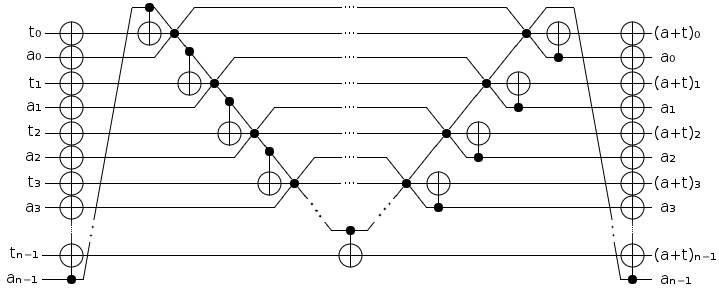
\includegraphics[width=\linewidth]{assets/inline-adder.png}
  \caption{\em Adder for input and target registers of the same size.
  Requires no ancilla, and uses $O(N)$ gates and depth.
  Based on \cite{van2004, takahashi2005}.}
  \label{fig:inlineadder}
\end{figure}

\begin{figure}
  \centering
  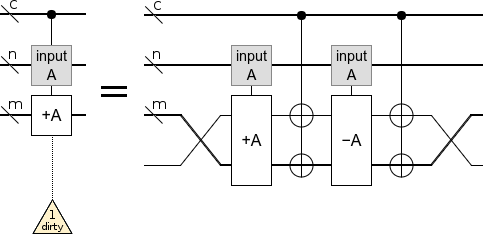
\includegraphics[width=\linewidth]{assets/controlled-addition.png}
  \caption{\em
  	Reducing controlled addition to uncontrolled addition.
  	Uses $O(N + C)$ gates and depth.
  }
  \label{fig:controlled-addition}
\end{figure}

Because this adder construction uses the input register as workspace, it breaks when the input and target registers differ in size.
When the input register is larger, the high bits of the input register can simply be ignored.
But, when the target register is larger, there is insufficient workspace and also the logical-negation trick that allowed the ancilla to be dirty breaks.

To work around the target register being larger, three tweaks are needed.
Each uses a controlled increment or decrement gate, which will be described in the next subsection.
(Note that, to avoid cyclic dependencies, the increment and decrement constructions will only use the same-register-size adder.)

First, the carry signal must be forwarded into the high part of the target register with a controlled increment instead of with a CNOT.
Second, to free the MSB of the input register for use as the carry signal, we add it into the target ahead of time with a controlled increment.
Finally, when the MSB is on instead of off its role as carry signal causes an extra increment of the target.
This extra increment is cancelled with a controlled decrement.
See the circuit diagram in figure \ref{fig:inline-adder-into-large}.

\begin{figure}
  \centering
  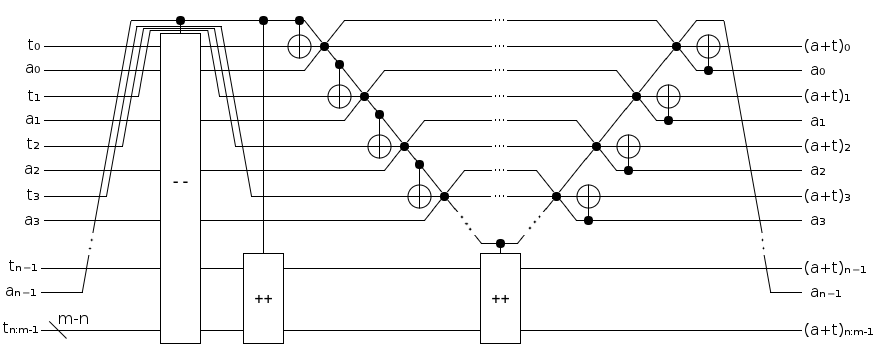
\includegraphics[width=\linewidth]{assets/inline-adder-into-large.png}
  \caption{\em
      Adder with target larger than source, using no ancilla.
      Uses $O(N)$ gates and depth.
      The increment and decrement gates all have at least one free wire to borrow as a dirty ancilla.}
  \label{fig:inline-adder-into-large}
\end{figure}

Another problem with using the input register as workspace appears when adding a constant offset into a target: there {\em isn't} an input register.
We use the construction from \cite{haner2016}, which works for constant offsets but increases the gate cost from $\Theta(n)$ to $\Theta(n \lg n)$ and also requires a dirty ancilla instead of no ancilla (unless using quantum operations).
See figure \ref{fig:controlled-offset}.
We note that our paper would have significantly fewer diagrams if offset and addition didn't have differing costs.


\subsection{Increment}

A register can be incremented by subtracting both $x$ and $\neg x = -x-1$ from it, for any $x$.
When $n$ dirty bits are available, $x$ can come from a register defined by those $n$ arbitrary bits, as shown in figure \ref{fig:increment-many-dirty}.

\begin{figure}
  \centering
  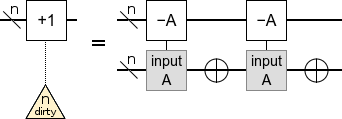
\includegraphics[width=\linewidth]{assets/increment-many-dirty.png}
  \caption{\em Subtracting $x$ and $-x-1$ from a register increments it. Requires $O(N)$ depth, size, and $N$ dirty ancilla.}
  \label{fig:increment-many-dirty}
\end{figure}

To improve from $n$ dirty bits to a single dirty bit, we break the increment operation into two halves.
A high half that is incremented only if all of the bottom bits are on, and a low half that is unconditionally incremented.
The low half can be incremented with the double-subtraction trick by borrowing the high half.
But the double-subtraction trick doesn't work on the high half, because the low half can't be borrowed when it is being used as a control.

To work around not being able to operate on the borrowed bits while using them as a control, start with the double-subtraction trick but change the second subtraction to an addition and conditionally toggle the target bits instead of the input bits.
When the condition isn't satisfied, the addition and subtraction will cancel each other.
When the condition is satisfied, the addition will be inverted into a subtraction, and both the subtraction and addition-turned-subtraction will fire, subtracting the input register from the target register twice.
However, because we are conditioning on the input bits all being on, we know the input must be -1.
Therefore the target was incremented by 2.
To halve the +2 into a +1, prepend a dirty least-significant-bit onto the target register as shown in \ref{fig:increment-odd}.

Because the adder/subtracter construction used by the incrementer in figure \ref{fig:increment-odd} requires the target and source registers to be the same size, the incrementer construction described so far only works on odd-sized registers.
For even-sized registers, another minor variation on the conditionally-invert-addition-into-subtraction-with-logical-negation technique is used.
That construction is shown in figure \ref{fig:increment-even}.

Increment gates can be efficiently controlled by using another invert-input-and-output trick.
See figures \ref{fig:controlled-increment-odd} and \ref{fig:controlled-increment-even}.

\begin{figure}
  \centering
  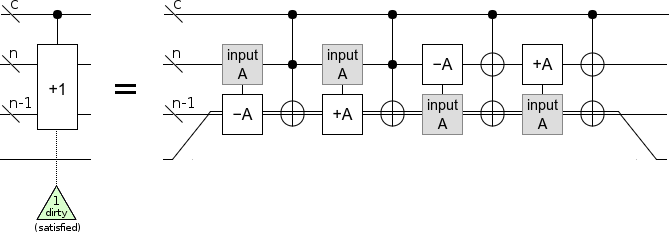
\includegraphics[width=\linewidth]{assets/controlled-increment-odd.png}
  \caption{\em Odd-sized $O(N)$ controlled increment with 1 dirty ancilla.}
  \label{fig:controlled-increment-odd}
\end{figure}

\begin{figure}
  \centering
  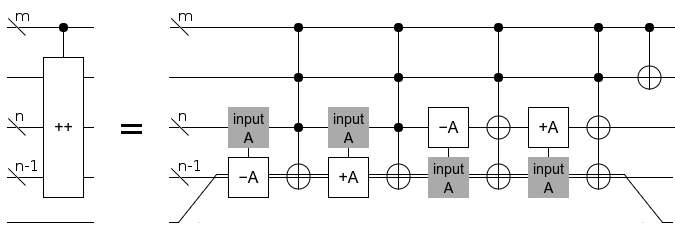
\includegraphics[width=\linewidth]{assets/controlled-increment-even.png}
  \caption{\em Even-sized $O(N)$ controlled increment with 1 dirty ancilla.}
  \label{fig:controlled-increment-even}
\end{figure}

\begin{figure}
  \centering
  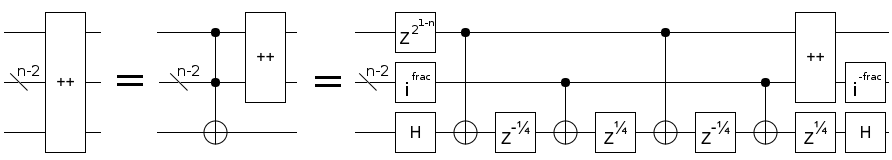
\includegraphics[width=\linewidth]{assets/ancilla-bootstrap.png}
  \caption{\em Bootstrapping a dirty ancilla out of an increment gate using quantum operations.
  The $i^{\text{frac}}$ gate is a ``phase gradient" operation that phases each computational basis state $|v\rangle$ by an amount proportional to $v/2^d$, where $d$ is the size of the register.
  In this case each state is phased by $e^{i \frac{\pi}{2} v/2^d}$.
  The phase gradient is implemented by a column of $Z^{2^{-k}}$ gates, .}
  \label{fig:bootstrap-ancilla}
\end{figure}


\subsection{Bit Swaps, Rotations, and Reversals}

Bit permuting operations are easy to overlook in circuits, because they can be emulated by re-labelling qubits.
But some of our circuit diagrams have used controlled bit permutations, requiring actual operations, so we provide the constructions for completeness.

\begin{figure}
  \centering
  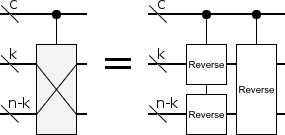
\includegraphics[width=\linewidth]{assets/controlled-bit-rotate.png}
  \caption{\em
    A controlled bit rotation / bit swap is three $O(N+C)$ controlled bit-reverses.
  }
  \label{fig:dependencies}
\end{figure}

\begin{figure}
  \centering
  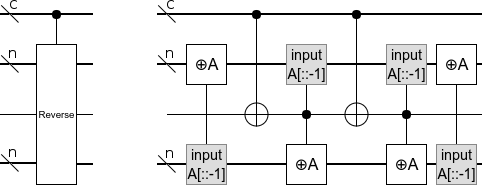
\includegraphics[width=\linewidth]{assets/controlled-reverse.png}
  \caption{\em
    An inline controlled bit order reversal using $O(N + C)$ gates.
    Each XOR operation is a series of CNOTs (note that the inputs have opposite endian-ness to the outputs).
    For reversals on an even number of bits, swap the center two bits beforehand then use one of them as the center workspace bit from this construction.
  }
  \label{fig:dependencies}
\end{figure}


\subsection{Multi-Nots}

Several of our constructions have used CNOTs with many controls and many targets.
To avoid paying the overhead of $c$ controls for every target, we use one big CNOT to toggle-control all the others. [[[ FIGURE ]]]
We then use a dirty ancilla (i.e. one of the other targets) to efficiently reduce the big CNOT into Toffolis.

\section{Overview and Improvements} \label{sec:costs}

In figure \ref{fig:dependencies} we show a dependency graph of the constructions discussed in this paper.
The total cost of period-finding, using this construction, is $O(n^3 \lg n)$ gates and $O(n^3)$ depth.
We perform $O(n)$ modular multiplications, each of which uses $O(n)$ modular additions and offsets, each of which uses $O(n \lg n)$ gates \cite{haner2016} and $O(n)$ depth.

We tested individual constructions in Quirk [[[ https://github.com/Strilanc/Quirk ]]] and the full construction down to Toffoli gates in ProjectQ [[[ https://github.com/ProjectQ-Framework/ProjectQ ]]] [[[ link to code ]]].

Our main improvements over previous constructions are 1) the use of pivot-flips for modular addition, 2) the use of bimultiplication for modular multiplication, and 3) the $O(n)$ incrementer requiring only a single dirty ancilla.

Previous modular addition constructions worked by temporarily storing an is-wraparound-needed comparison in a clean ancilla \cite{takahashi2006, haner2016}.
Pivot flips also require an ancilla (two, actually), but the ancilla can be dirty and, in the context of period-finding, there's always qubits available to borrow whenever a pivot-flip is needed.
This improvement saves a qubit, reducing the total number of qubits required for period finding from $2n+2$ to $2n+1$.

Previous modular multiplication constructions required a clean ancilla register \cite{haner2016}, where any garbage in the ancilla register would have infected the target register and trashed it.
We deal with the trash with an extra multiply-accumulate per modular multiplication, and cancel the overall effects on the ancilla register with a clean-up multiplication informed by measuring the main register at the end of the circuit.
This improvement allows $n-1$ of the qubits in the ancilla register  to be dirty (only the MSB must be zero; to ensure the register's value is in range).

Previous published incrementers (not counting a rough unpublished version of our construction \cite{gidney2015} being cited by \cite{haner2016}) required either $O(n^2)$ gates or $O(n)$ ancilla \cite{draper2000, barenco1995}.
Our classical incrementer constructions use $O(n)$ gates and a single dirty ancilla.
Note that, for classical reversible computation, 1 dirty ancilla is optimal.
The parity of the permutation performed by an increment operation is odd, but the parity of the permutation performed by any classical gate that doesn't cover the entire circuit is even.
With quantum operations, we achieve zero ancilla and $O(n)$ gates (see figure \ref{fig:bootstrap-ancilla}).

\begin{figure}
  \centering
  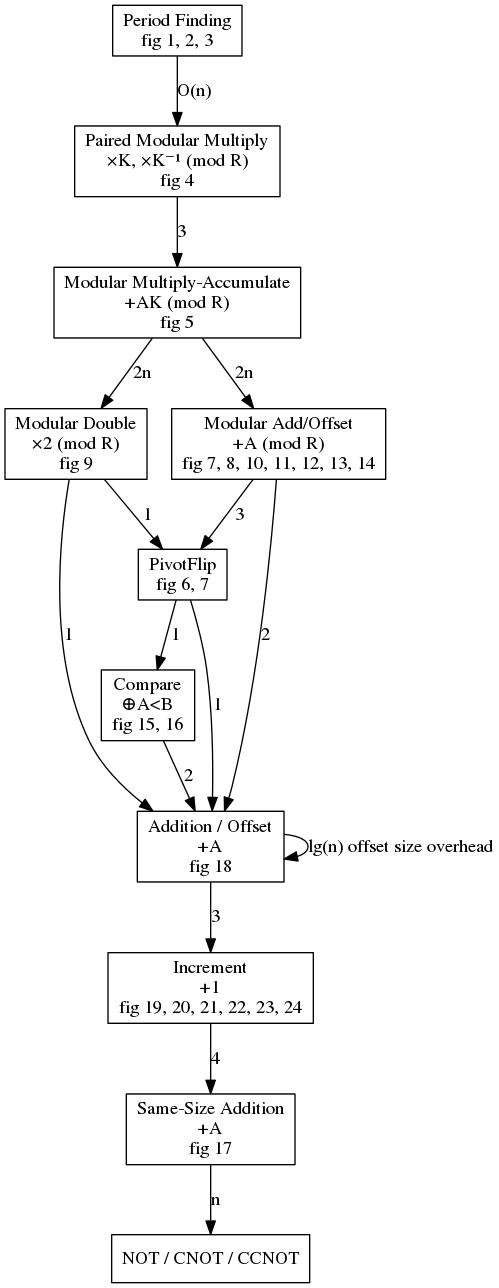
\includegraphics[height=17.3cm]{assets/dependencies.png}
  \caption{\em
    Graph of non-trivial dependencies between constructions, from period finding to fixed-size gates.
    Edges are labelled by an upper bound on how many times the target is used by the source.
  }
  \label{fig:dependencies}
\end{figure}


\section{Conclusion} \label{sec:conclusion}

We presented Toffoli-based arithmetic circuits that reduce the smallest known number of qubits required to perform Shor's algorithm by 1, and allowed an additional $n-1$ qubits to be dirty.

\bibliographystyle{plain}
\bibliography{citations}

\section{Temporary Test Circuit Links}

Convenience links for myself when checking that things work.

\href
{http://algassert.com/quirk#circuit=%7B%22cols%22%3A%5B%5B%22X%22%2C%22X%22%2C%22X%22%2C%22X%22%2C%22%E2%80%A2%22%2C%22X%22%2C%22X%22%2C%22X%22%2C%22X%22%2C%22X%22%5D%2C%5B%22%E2%80%A2%22%2C1%2C1%2C1%2C1%2C%22X%22%5D%2C%5B%22Swap%22%2C1%2C1%2C1%2C%22Swap%22%2C%22%E2%80%A2%22%5D%2C%5B1%2C%22%E2%80%A2%22%2C1%2C1%2C1%2C1%2C%22X%22%5D%2C%5B1%2C%22Swap%22%2C1%2C1%2C%22Swap%22%2C1%2C%22%E2%80%A2%22%5D%2C%5B1%2C1%2C%22%E2%80%A2%22%2C1%2C1%2C1%2C1%2C%22X%22%5D%2C%5B1%2C1%2C%22Swap%22%2C1%2C%22Swap%22%2C1%2C1%2C%22%E2%80%A2%22%5D%2C%5B1%2C1%2C1%2C%22%E2%80%A2%22%2C1%2C1%2C1%2C1%2C%22X%22%5D%2C%5B1%2C1%2C1%2C%22Swap%22%2C%22Swap%22%2C1%2C1%2C1%2C%22%E2%80%A2%22%5D%2C%5B1%2C1%2C1%2C1%2C%22%E2%80%A2%22%2C1%2C1%2C1%2C1%2C%22X%22%5D%2C%5B1%2C1%2C1%2C%22Swap%22%2C%22Swap%22%2C1%2C1%2C1%2C%22%E2%80%A2%22%5D%2C%5B1%2C1%2C1%2C1%2C%22%E2%80%A2%22%2C1%2C1%2C1%2C%22X%22%5D%2C%5B1%2C1%2C%22Swap%22%2C1%2C%22Swap%22%2C1%2C1%2C%22%E2%80%A2%22%5D%2C%5B1%2C1%2C1%2C1%2C%22%E2%80%A2%22%2C1%2C1%2C%22X%22%5D%2C%5B1%2C%22Swap%22%2C1%2C1%2C%22Swap%22%2C1%2C%22%E2%80%A2%22%5D%2C%5B1%2C1%2C1%2C1%2C%22%E2%80%A2%22%2C1%2C%22X%22%5D%2C%5B%22Swap%22%2C1%2C1%2C1%2C%22Swap%22%2C%22%E2%80%A2%22%5D%2C%5B1%2C1%2C1%2C1%2C%22%E2%80%A2%22%2C%22X%22%5D%2C%5B%22X%22%2C%22X%22%2C%22X%22%2C%22X%22%2C%22%E2%80%A2%22%2C%22X%22%2C%22X%22%2C%22X%22%2C%22X%22%2C%22X%22%5D%5D%7D}
{5+5-bit inline adder}
(or \href
{http://algassert.com/quirk#circuit=%7B%22cols%22%3A%5B%5B%22Counting10%22%5D%2C%5B%22QFT7%22%5D%2C%5B1%2C1%2C1%2C%22QFT7%22%5D%2C%5B%22%E2%80%A6%22%5D%2C%5B%22%E2%80%A6%22%5D%2C%5B%22X%22%2C%22X%22%2C%22X%22%2C%22X%22%2C%22%E2%80%A2%22%2C%22X%22%2C%22X%22%2C%22X%22%2C%22X%22%2C%22X%22%5D%2C%5B%22%E2%80%A2%22%2C1%2C1%2C1%2C1%2C%22X%22%5D%2C%5B%22Swap%22%2C1%2C1%2C1%2C%22Swap%22%2C%22%E2%80%A2%22%5D%2C%5B1%2C%22%E2%80%A2%22%2C1%2C1%2C1%2C1%2C%22X%22%5D%2C%5B1%2C%22Swap%22%2C1%2C1%2C%22Swap%22%2C1%2C%22%E2%80%A2%22%5D%2C%5B1%2C1%2C%22%E2%80%A2%22%2C1%2C1%2C1%2C1%2C%22X%22%5D%2C%5B1%2C1%2C%22Swap%22%2C1%2C%22Swap%22%2C1%2C1%2C%22%E2%80%A2%22%5D%2C%5B1%2C1%2C1%2C%22%E2%80%A2%22%2C1%2C1%2C1%2C1%2C%22X%22%5D%2C%5B1%2C1%2C1%2C%22Swap%22%2C%22Swap%22%2C1%2C1%2C1%2C%22%E2%80%A2%22%5D%2C%5B1%2C1%2C1%2C1%2C%22%E2%80%A2%22%2C1%2C1%2C1%2C1%2C%22X%22%5D%2C%5B1%2C1%2C1%2C%22Swap%22%2C%22Swap%22%2C1%2C1%2C1%2C%22%E2%80%A2%22%5D%2C%5B1%2C1%2C1%2C1%2C%22%E2%80%A2%22%2C1%2C1%2C1%2C%22X%22%5D%2C%5B1%2C1%2C%22Swap%22%2C1%2C%22Swap%22%2C1%2C1%2C%22%E2%80%A2%22%5D%2C%5B1%2C1%2C1%2C1%2C%22%E2%80%A2%22%2C1%2C1%2C%22X%22%5D%2C%5B1%2C%22Swap%22%2C1%2C1%2C%22Swap%22%2C1%2C%22%E2%80%A2%22%5D%2C%5B1%2C1%2C1%2C1%2C%22%E2%80%A2%22%2C1%2C%22X%22%5D%2C%5B%22Swap%22%2C1%2C1%2C1%2C%22Swap%22%2C%22%E2%80%A2%22%5D%2C%5B1%2C1%2C1%2C1%2C%22%E2%80%A2%22%2C%22X%22%5D%2C%5B%22X%22%2C%22X%22%2C%22X%22%2C%22X%22%2C%22%E2%80%A2%22%2C%22X%22%2C%22X%22%2C%22X%22%2C%22X%22%2C%22X%22%5D%2C%5B%22%E2%80%A6%22%5D%2C%5B%22%E2%80%A6%22%5D%2C%5B%22inputA5%22%2C1%2C1%2C1%2C1%2C%22%2B%3DA5%22%5D%2C%5B1%2C1%2C1%2C%22QFT%E2%80%A07%22%5D%2C%5B%22QFT%E2%80%A07%22%5D%2C%5B%22Uncounting10%22%5D%5D%7D}
{with test harness})

\href
{http://algassert.com/quirk#circuit=%7B%22cols%22%3A%5B%5B%22inputA4%22%2C1%2C1%2C1%2C%22-%3DA4%22%5D%2C%5B%22X%22%2C%22X%22%2C%22X%22%2C%22X%22%5D%2C%5B%22inputA4%22%2C1%2C1%2C1%2C%22-%3DA4%22%5D%2C%5B%22X%22%2C%22X%22%2C%22X%22%2C%22X%22%5D%5D%7D}
{4-bit incrementer w/ 4 dirty}

\href
{http://algorithmicassertions.com/quirk#circuit=%7B%22cols%22%3A%5B%5B1%2C1%2C1%2C1%2C1%2C%22%3C%3C4%22%5D%2C%5B1%2C%22inputA4%22%2C1%2C1%2C1%2C%22-%3DA4%22%5D%2C%5B%22%E2%80%A2%22%2C%22%E2%80%A2%22%2C%22%E2%80%A2%22%2C%22%E2%80%A2%22%2C%22%E2%80%A2%22%2C%22X%22%2C%22X%22%2C%22X%22%2C%22X%22%5D%2C%5B1%2C%22inputA4%22%2C1%2C1%2C1%2C%22%2B%3DA4%22%5D%2C%5B%22%E2%80%A2%22%2C%22%E2%80%A2%22%2C%22%E2%80%A2%22%2C%22%E2%80%A2%22%2C%22%E2%80%A2%22%2C%22X%22%2C%22X%22%2C%22X%22%2C%22X%22%5D%2C%5B1%2C%22-%3DA4%22%2C1%2C1%2C1%2C%22inputA4%22%5D%2C%5B%22%E2%80%A2%22%2C%22X%22%2C%22X%22%2C%22X%22%2C%22X%22%2C%22X%22%2C%22X%22%2C%22X%22%2C%22X%22%5D%2C%5B1%2C%22%2B%3DA4%22%2C1%2C1%2C1%2C%22inputA4%22%5D%2C%5B%22%E2%80%A2%22%2C%22X%22%2C%22X%22%2C%22X%22%2C%22X%22%2C%22X%22%2C%22X%22%2C%22X%22%2C%22X%22%5D%2C%5B%22X%22%5D%2C%5B1%2C1%2C1%2C1%2C1%2C%22%3E%3E4%22%5D%5D%7D}
{8-bit incrementer w/ 1 dirty}
(or \href
{http://algorithmicassertions.com/quirk#circuit=%7B%22cols%22%3A%5B%5B%22Counting9%22%5D%2C%5B%22QFT6%22%5D%2C%5B1%2C1%2C1%2C%22QFT6%22%5D%2C%5B%22%E2%80%A6%22%5D%2C%5B%22%E2%80%A6%22%5D%2C%5B1%2C1%2C1%2C1%2C1%2C%22%3C%3C4%22%5D%2C%5B1%2C%22inputA4%22%2C1%2C1%2C1%2C%22-%3DA4%22%5D%2C%5B%22%E2%80%A2%22%2C%22%E2%80%A2%22%2C%22%E2%80%A2%22%2C%22%E2%80%A2%22%2C%22%E2%80%A2%22%2C%22X%22%2C%22X%22%2C%22X%22%2C%22X%22%5D%2C%5B1%2C%22inputA4%22%2C1%2C1%2C1%2C%22%2B%3DA4%22%5D%2C%5B%22%E2%80%A2%22%2C%22%E2%80%A2%22%2C%22%E2%80%A2%22%2C%22%E2%80%A2%22%2C%22%E2%80%A2%22%2C%22X%22%2C%22X%22%2C%22X%22%2C%22X%22%5D%2C%5B1%2C%22-%3DA4%22%2C1%2C1%2C1%2C%22inputA4%22%5D%2C%5B%22%E2%80%A2%22%2C%22X%22%2C%22X%22%2C%22X%22%2C%22X%22%2C%22X%22%2C%22X%22%2C%22X%22%2C%22X%22%5D%2C%5B1%2C%22%2B%3DA4%22%2C1%2C1%2C1%2C%22inputA4%22%5D%2C%5B%22%E2%80%A2%22%2C%22X%22%2C%22X%22%2C%22X%22%2C%22X%22%2C%22X%22%2C%22X%22%2C%22X%22%2C%22X%22%5D%2C%5B%22X%22%5D%2C%5B1%2C1%2C1%2C1%2C1%2C%22%3E%3E4%22%5D%2C%5B%22%E2%80%A6%22%5D%2C%5B%22%E2%80%A6%22%5D%2C%5B%22dec8%22%5D%2C%5B1%2C1%2C1%2C%22QFT%E2%80%A06%22%5D%2C%5B%22QFT%E2%80%A06%22%5D%2C%5B%22Uncounting9%22%5D%5D%7D}
{with test harness})

\href
{http://algorithmicassertions.com/quirk#circuit=%7B%22cols%22%3A%5B%5B1%2C1%2C1%2C1%2C1%2C%22%3C%3C5%22%5D%2C%5B%22inputA5%22%2C1%2C1%2C1%2C1%2C%22-%3DA5%22%5D%2C%5B%22%E2%80%A2%22%2C%22%E2%80%A2%22%2C%22%E2%80%A2%22%2C%22%E2%80%A2%22%2C%22%E2%80%A2%22%2C%22X%22%2C%22X%22%2C%22X%22%2C%22X%22%2C%22X%22%5D%2C%5B%22inputA5%22%2C1%2C1%2C1%2C1%2C%22%2B%3DA5%22%5D%2C%5B%22%E2%80%A2%22%2C%22%E2%80%A2%22%2C%22%E2%80%A2%22%2C%22%E2%80%A2%22%2C%22%E2%80%A2%22%2C%22X%22%2C%22X%22%2C%22X%22%2C%22X%22%2C%22X%22%5D%2C%5B%22-%3DA5%22%2C1%2C1%2C1%2C1%2C%22inputA5%22%5D%2C%5B1%2C1%2C1%2C1%2C1%2C%22X%22%2C%22X%22%2C%22X%22%2C%22X%22%2C%22X%22%5D%2C%5B%22-%3DA5%22%2C1%2C1%2C1%2C1%2C%22inputA5%22%5D%2C%5B1%2C1%2C1%2C1%2C1%2C%22X%22%2C%22X%22%2C%22X%22%2C%22X%22%2C%22X%22%5D%2C%5B1%2C1%2C1%2C1%2C1%2C%22%3E%3E5%22%5D%5D%7D}
{9-bit incrementer w/ 1 dirty}
(or \href
{http://algorithmicassertions.com/quirk#circuit=%7B%22cols%22%3A%5B%5B%22Counting10%22%5D%2C%5B%22QFT7%22%5D%2C%5B1%2C1%2C1%2C%22QFT7%22%5D%2C%5B%22%E2%80%A6%22%5D%2C%5B%22%E2%80%A6%22%5D%2C%5B1%2C1%2C1%2C1%2C1%2C%22%3C%3C5%22%5D%2C%5B%22inputA5%22%2C1%2C1%2C1%2C1%2C%22-%3DA5%22%5D%2C%5B%22%E2%80%A2%22%2C%22%E2%80%A2%22%2C%22%E2%80%A2%22%2C%22%E2%80%A2%22%2C%22%E2%80%A2%22%2C%22X%22%2C%22X%22%2C%22X%22%2C%22X%22%2C%22X%22%5D%2C%5B%22inputA5%22%2C1%2C1%2C1%2C1%2C%22%2B%3DA5%22%5D%2C%5B%22%E2%80%A2%22%2C%22%E2%80%A2%22%2C%22%E2%80%A2%22%2C%22%E2%80%A2%22%2C%22%E2%80%A2%22%2C%22X%22%2C%22X%22%2C%22X%22%2C%22X%22%2C%22X%22%5D%2C%5B%22-%3DA5%22%2C1%2C1%2C1%2C1%2C%22inputA5%22%5D%2C%5B1%2C1%2C1%2C1%2C1%2C%22X%22%2C%22X%22%2C%22X%22%2C%22X%22%2C%22X%22%5D%2C%5B%22-%3DA5%22%2C1%2C1%2C1%2C1%2C%22inputA5%22%5D%2C%5B1%2C1%2C1%2C1%2C1%2C%22X%22%2C%22X%22%2C%22X%22%2C%22X%22%2C%22X%22%5D%2C%5B1%2C1%2C1%2C1%2C1%2C%22%3E%3E5%22%5D%2C%5B%22%E2%80%A6%22%5D%2C%5B%22%E2%80%A6%22%5D%2C%5B%22dec9%22%5D%2C%5B1%2C1%2C1%2C%22QFT%E2%80%A07%22%5D%2C%5B%22QFT%E2%80%A07%22%5D%2C%5B%22Uncounting10%22%5D%5D%7D}
{with test harness})

\href
{http://algorithmicassertions.com/quirk#circuit=%7B%22cols%22%3A%5B%5B%22Z%5E%E2%85%9F%E2%82%81%E2%82%86%22%2C%22Z%5E%E2%85%9F%E2%82%81%E2%82%86%22%2C%22Z%5E%E2%85%9B%22%2C%22Z%5E%C2%BC%22%2C%22H%22%5D%2C%5B%22%E2%80%A2%22%2C1%2C1%2C1%2C%22X%22%5D%2C%5B1%2C1%2C1%2C1%2C%22Z%5E-%C2%BC%22%5D%2C%5B1%2C%22%E2%80%A2%22%2C%22%E2%80%A2%22%2C%22%E2%80%A2%22%2C%22X%22%5D%2C%5B1%2C1%2C1%2C1%2C%22Z%5E%C2%BC%22%5D%2C%5B%22%E2%80%A2%22%2C1%2C1%2C1%2C%22X%22%5D%2C%5B1%2C1%2C1%2C1%2C%22Z%5E-%C2%BC%22%5D%2C%5B1%2C%22%E2%80%A2%22%2C%22%E2%80%A2%22%2C%22%E2%80%A2%22%2C%22X%22%5D%2C%5B%22inc4%22%2C1%2C1%2C1%2C%22Z%5E%C2%BC%22%5D%2C%5B1%2C%22Z%5E-%E2%85%9F%E2%82%81%E2%82%86%22%2C%22Z%5E-%E2%85%9B%22%2C%22Z%5E-%C2%BC%22%2C%22H%22%5D%5D%7D}
{Quantum incrementer ancilla bootstrap}

NOTE: have to open these next ones against local version, because online version doesn't have the comparison gates

\href
{http://algassert.com/quirk#circuit=%7B%22cols%22%3A%5B%5B%22inputA4%22%2C1%2C1%2C1%2C%22inputB4%22%2C1%2C1%2C1%2C%22%5EA%3EB%22%5D%2C%5B%22inputA4%22%2C1%2C1%2C1%2C%22-%3DA4%22%2C1%2C1%2C1%2C%22%E2%80%A2%22%5D%2C%5B1%2C1%2C1%2C1%2C%22X%22%2C%22X%22%2C%22X%22%2C%22X%22%2C%22%E2%80%A2%22%5D%2C%5B%22inputA4%22%2C1%2C1%2C1%2C%22inputB4%22%2C1%2C1%2C1%2C%22%5EA%3EB%22%5D%2C%5B%22inputA4%22%2C1%2C1%2C1%2C%22-%3DA4%22%2C1%2C1%2C1%2C%22%E2%80%A2%22%5D%2C%5B1%2C1%2C1%2C1%2C%22X%22%2C%22X%22%2C%22X%22%2C%22X%22%2C%22%E2%80%A2%22%5D%5D%7D}
{4+4-Bit $<$ PivotFlip}
(or \href
{http://algassert.com/quirk#circuit=%7B%22cols%22%3A%5B%5B1%2C1%2C1%2C1%2C%22H%22%2C%22H%22%2C%22H%22%2C%22H%22%5D%2C%5B%22Counting4%22%2C1%2C1%2C1%2C%22inputA4%22%2C1%2C1%2C1%2C%22%2B%3DA4%22%2C1%2C1%2C1%2C%22X%5Et%22%5D%2C%5B1%2C1%2C1%2C1%2C1%2C1%2C1%2C1%2C%22%3C%3C5%22%5D%2C%5B%22%E2%80%A6%22%5D%2C%5B%22%E2%80%A6%22%5D%2C%5B%22inputA4%22%2C1%2C1%2C1%2C%22inputB4%22%2C1%2C1%2C1%2C%22%5EA%3EB%22%5D%2C%5B%22inputA4%22%2C1%2C1%2C1%2C%22-%3DA4%22%2C1%2C1%2C1%2C%22%E2%80%A2%22%5D%2C%5B1%2C1%2C1%2C1%2C%22X%22%2C%22X%22%2C%22X%22%2C%22X%22%2C%22%E2%80%A2%22%5D%2C%5B%22inputA4%22%2C1%2C1%2C1%2C%22inputB4%22%2C1%2C1%2C1%2C%22%5EA%3EB%22%5D%2C%5B%22inputA4%22%2C1%2C1%2C1%2C%22-%3DA4%22%2C1%2C1%2C1%2C%22%E2%80%A2%22%5D%2C%5B1%2C1%2C1%2C1%2C%22X%22%2C%22X%22%2C%22X%22%2C%22X%22%2C%22%E2%80%A2%22%5D%2C%5B%22%E2%80%A6%22%5D%2C%5B%22%E2%80%A6%22%5D%2C%5B1%2C1%2C1%2C1%2C1%2C1%2C1%2C1%2C%22%3E%3E5%22%5D%2C%5B1%2C1%2C1%2C1%2C1%2C1%2C1%2C1%2C1%2C1%2C1%2C1%2C%22X%5E-t%22%5D%2C%5B%22Chance4%22%2C1%2C1%2C1%2C%22Amps8%22%2C1%2C1%2C1%2C1%2C1%2C1%2C1%2C%22Chance%22%5D%5D%7D}
{with test harness})

\href
{http://algassert.com/quirk#circuit=%7B%22cols%22%3A%5B%5B%22inputA4%22%2C1%2C1%2C1%2C%22inputB4%22%2C1%2C1%2C1%2C%22%5EA%3E%3DB%22%5D%2C%5B%22inputA4%22%2C1%2C1%2C1%2C%22-%3DA4%22%2C1%2C1%2C1%2C%22%E2%80%A2%22%5D%2C%5B1%2C1%2C1%2C1%2C%22dec4%22%2C1%2C1%2C1%2C%22%E2%80%A2%22%5D%2C%5B1%2C1%2C1%2C1%2C%22X%22%2C%22X%22%2C%22X%22%2C%22X%22%2C%22%E2%80%A2%22%5D%2C%5B%22inputA4%22%2C1%2C1%2C1%2C%22inputB4%22%2C1%2C1%2C1%2C%22%5EA%3E%3DB%22%5D%2C%5B%22inputA4%22%2C1%2C1%2C1%2C%22-%3DA4%22%2C1%2C1%2C1%2C%22%E2%80%A2%22%5D%2C%5B1%2C1%2C1%2C1%2C%22dec4%22%2C1%2C1%2C1%2C%22%E2%80%A2%22%5D%2C%5B1%2C1%2C1%2C1%2C%22X%22%2C%22X%22%2C%22X%22%2C%22X%22%2C%22%E2%80%A2%22%5D%5D%7D}
{4+4-Bit $\leq$ PivotFlip}
(or \href
{http://algassert.com/quirk#circuit=%7B%22cols%22%3A%5B%5B1%2C1%2C1%2C1%2C%22H%22%2C%22H%22%2C%22H%22%2C%22H%22%5D%2C%5B%22Counting4%22%2C1%2C1%2C1%2C%22inputA4%22%2C1%2C1%2C1%2C%22%2B%3DA4%22%2C1%2C1%2C1%2C%22X%5Et%22%5D%2C%5B1%2C1%2C1%2C1%2C1%2C1%2C1%2C1%2C%22%3C%3C5%22%5D%2C%5B%22%E2%80%A6%22%5D%2C%5B%22%E2%80%A6%22%5D%2C%5B%22inputA4%22%2C1%2C1%2C1%2C%22inputB4%22%2C1%2C1%2C1%2C%22%5EA%3E%3DB%22%5D%2C%5B%22inputA4%22%2C1%2C1%2C1%2C%22-%3DA4%22%2C1%2C1%2C1%2C%22%E2%80%A2%22%5D%2C%5B1%2C1%2C1%2C1%2C%22dec4%22%2C1%2C1%2C1%2C%22%E2%80%A2%22%5D%2C%5B1%2C1%2C1%2C1%2C%22X%22%2C%22X%22%2C%22X%22%2C%22X%22%2C%22%E2%80%A2%22%5D%2C%5B%22inputA4%22%2C1%2C1%2C1%2C%22inputB4%22%2C1%2C1%2C1%2C%22%5EA%3E%3DB%22%5D%2C%5B%22inputA4%22%2C1%2C1%2C1%2C%22-%3DA4%22%2C1%2C1%2C1%2C%22%E2%80%A2%22%5D%2C%5B1%2C1%2C1%2C1%2C%22dec4%22%2C1%2C1%2C1%2C%22%E2%80%A2%22%5D%2C%5B1%2C1%2C1%2C1%2C%22X%22%2C%22X%22%2C%22X%22%2C%22X%22%2C%22%E2%80%A2%22%5D%2C%5B%22%E2%80%A6%22%5D%2C%5B%22%E2%80%A6%22%5D%2C%5B1%2C1%2C1%2C1%2C1%2C1%2C1%2C1%2C%22%3E%3E5%22%5D%2C%5B1%2C1%2C1%2C1%2C1%2C1%2C1%2C1%2C1%2C1%2C1%2C1%2C%22X%5E-t%22%5D%2C%5B%22Chance4%22%2C1%2C1%2C1%2C%22Amps8%22%2C1%2C1%2C1%2C1%2C1%2C1%2C1%2C%22Chance%22%5D%5D%7D}
{with test harness})

\href
{http://algassert.com/quirk#circuit=%7B%22cols%22%3A%5B%5B1%2C1%2C1%2C1%2C1%2C1%2C1%2C1%2C%22inc4%22%5D%2C%5B%22X%22%2C1%2C1%2C%22X%22%2C%22Counting4%22%2C1%2C1%2C1%2C%22QFT4%22%5D%2C%5B1%2C1%2C1%2C1%2C1%2C1%2C1%2C1%2C%22inputA4%22%2C1%2C1%2C1%2C%22%2B%3DA4%22%5D%2C%5B%22Chance4%22%2C1%2C1%2C1%2C%22Chance4%22%2C1%2C1%2C1%2C%22Chance4%22%5D%2C%5B%22%E2%80%A6%22%5D%2C%5B%22%E2%80%A6%22%5D%2C%5B%22inputA4%22%2C1%2C1%2C1%2C%22%2B%3DA4%22%5D%2C%5B1%2C1%2C1%2C1%2C%22X%22%2C%22X%22%2C%22X%22%2C%22X%22%5D%2C%5B1%2C1%2C1%2C1%2C%22inc4%22%5D%2C%5B1%2C1%2C1%2C1%2C%22inputA4%22%2C1%2C1%2C1%2C%22Flip%3CA4%22%5D%2C%5B1%2C1%2C1%2C1%2C%22dec4%22%5D%2C%5B1%2C1%2C1%2C1%2C%22X%22%2C%22X%22%2C%22X%22%2C%22X%22%5D%2C%5B%22inputA4%22%2C1%2C1%2C1%2C1%2C1%2C1%2C1%2C%22Flip%3CA4%22%5D%2C%5B%22inputA4%22%2C1%2C1%2C1%2C%22%2B%3DA4%22%5D%2C%5B1%2C1%2C1%2C1%2C%22inputA4%22%2C1%2C1%2C1%2C%22Flip%3CA4%22%5D%2C%5B%22%E2%80%A6%22%5D%2C%5B%22%E2%80%A6%22%5D%2C%5B%22Chance4%22%2C1%2C1%2C1%2C%22Chance4%22%2C1%2C1%2C1%2C%22Amps8%22%5D%2C%5B%5D%2C%5B%5D%2C%5B%5D%2C%5B%5D%2C%5B%5D%2C%5B%5D%2C%5B%5D%2C%5B1%2C1%2C1%2C1%2C1%2C1%2C1%2C1%2C%22%7C0%E2%9F%A9%E2%9F%A80%7C%22%5D%2C%5B%22inputB4%22%2C1%2C1%2C1%2C%22inputA4%22%2C1%2C1%2C1%2C%22%5EA%3E%3DB%22%5D%2C%5B1%2C1%2C1%2C1%2C1%2C1%2C1%2C1%2C%22Chance%22%5D%2C%5B1%2C1%2C1%2C1%2C1%2C1%2C1%2C1%2C%22~a82g%22%5D%5D%2C%22gates%22%3A%5B%7B%22id%22%3A%22~a82g%22%2C%22name%22%3A%22IGNORE%22%2C%22matrix%22%3A%22%7B%7B1%2C0%7D%2C%7B0%2C1%7D%7D%22%7D%5D%7D}
{Modular Addition with test Harness}

\end{document}
